\section{Consulta de Datos: \texttt{SELECT}}

La instrucción \texttt{SELECT} es, sin duda, la más utilizada y la
más rica en posibilidades de todo el lenguaje SQL.
Su propósito es \textbf{consultar} datos: extraer filas de una o
varias tablas, aplicarles filtros, transformaciones y ordenamientos,
y devolver un resultado tabular.
A diferencia de \texttt{INSERT}, \texttt{UPDATE} o \texttt{DELETE},
\texttt{SELECT} es una operación de \textbf{sólo lectura}: nunca
modifica los datos almacenados.

%--------------------------------------------------------------
\subsection{Sintaxis completa y cláusulas}
%--------------------------------------------------------------

La sintaxis formal de \texttt{SELECT} en MySQL/SQL estándar es la
siguiente.
Las partes entre corchetes \texttt{[ ]} son opcionales; las palabras
en mayúsculas son palabras reservadas de SQL:

\begin{lstlisting}[caption={Sintaxis completa de SELECT.}]
SELECT  [ALL | DISTINCT | DISTINCTROW]
        lista_de_columnas | *
FROM    nombre_tabla  [[AS] alias_tabla]
[WHERE      condicion]
[GROUP BY   columna [ASC | DESC], ...]
[HAVING     condicion_de_grupo]
[ORDER BY   columna [ASC | DESC], ...]
[LIMIT      numero_de_filas  [OFFSET desplazamiento]];
\end{lstlisting}

Cada cláusula tiene un rol preciso dentro de la consulta.
La \cref{tab:clausulas-select} resume su función y el orden en que
el SGBD las \textit{evalúa} internamente (que no siempre coincide
con el orden en que se escriben):

\begin{table}[H]
\centering
\small
\renewcommand{\arraystretch}{1.4}
\begin{tabularx}{\linewidth}{@{} l c X @{}}
\toprule
\textbf{Cláusula} & \textbf{Orden eval.} & \textbf{Función} \\
\midrule
\texttt{FROM}     & 1 & Determina la(s) tabla(s) fuente de datos. \\
\texttt{WHERE}    & 2 & Filtra filas \textit{antes} de agrupar. \\
\texttt{GROUP BY} & 3 & Agrupa filas con valores iguales en las columnas indicadas. \\
\texttt{HAVING}   & 4 & Filtra grupos \textit{después} de agrupar. \\
\texttt{SELECT}   & 5 & Proyecta (selecciona) las columnas del resultado. \\
\texttt{DISTINCT} & 6 & Elimina filas duplicadas del resultado proyectado. \\
\texttt{ORDER BY} & 7 & Ordena el resultado final. \\
\texttt{LIMIT}    & 8 & Recorta el número de filas devueltas. \\
\bottomrule
\end{tabularx}
\caption{Cláusulas de \texttt{SELECT} y su orden de evaluación interno.}
\label{tab:clausulas-select}
\end{table}

\begin{nota}
El orden de \textbf{escritura} de las cláusulas es fijo y debe
respetarse exactamente como aparece en la sintaxis de arriba.
Sin embargo, el SGBD las \textbf{evalúa} en un orden diferente
(véase \cref{tab:clausulas-select}).
Esto explica, por ejemplo, por qué no se puede usar un alias
definido en \texttt{SELECT} dentro de la cláusula \texttt{WHERE}:
\texttt{WHERE} se evalúa \textit{antes} de que exista el alias.
\end{nota}

%--------------------------------------------------------------
\subsection{Tabla de ejemplo}
%--------------------------------------------------------------

Para ilustrar todos los ejemplos de esta sección usaremos una tabla
llamada \texttt{empleados} con la siguiente estructura y datos:

\begin{lstlisting}[caption={Creación e inicialización de la tabla \texttt{empleados}.}]
CREATE TABLE empleados (
    id          INT          PRIMARY KEY AUTO_INCREMENT,
    nombre      VARCHAR(60)  NOT NULL,
    departamento VARCHAR(40) NOT NULL,
    cargo       VARCHAR(40)  NOT NULL,
    salario     DECIMAL(10,2) NOT NULL,
    fecha_ingreso DATE        NOT NULL
);

INSERT INTO empleados (nombre, departamento, cargo, salario, fecha_ingreso) VALUES
('Ana García',      'Ventas',     'Gerente',    55000.00, '2018-03-15'),
('Luis Herrera',    'Ventas',     'Analista',   32000.00, '2020-07-01'),
('Sofía Ramírez',   'TI',         'Desarrolladora', 48000.00, '2019-11-20'),
('Carlos Mendoza',  'TI',         'DBA',        51000.00, '2017-05-10'),
('Elena Torres',    'RRHH',       'Coordinadora', 38000.00, '2021-02-28'),
('Marco Villanueva','Ventas',     'Analista',   31000.00, '2022-09-05'),
('Patricia Luna',   'TI',         'Desarrolladora', 47000.00, '2020-04-14'),
('Roberto Salas',   'RRHH',       'Gerente',    52000.00, '2016-08-22'),
('Diana Castillo',  'Finanzas',   'Analista',   39000.00, '2023-01-10'),
('Javier Moreno',   'Finanzas',   'Gerente',    58000.00, '2015-06-30');
\end{lstlisting}

%--------------------------------------------------------------
\subsection{Proyección de columnas: \texttt{SELECT *} y columnas específicas}
%--------------------------------------------------------------
\clearpage
La \textbf{proyección} es la operación de elegir qué columnas
aparecerán en el resultado.
El asterisco \texttt{*} es un comodín que significa
\textit{``todas las columnas''}.

\begin{lstlisting}[caption={Seleccionar todas las columnas.}]
-- Devuelve todas las columnas de todos los empleados
SELECT *
FROM empleados;
\end{lstlisting}

\begin{lstlisting}[caption={Seleccionar columnas específicas.}]
-- Sólo nombre, departamento y salario
SELECT nombre, departamento, salario
FROM empleados;
\end{lstlisting}

\begin{nota}
En producción se recomienda \textbf{evitar} \texttt{SELECT *} porque:
(1) transfiere columnas innecesarias por la red,
(2) si alguien agrega una columna sensible a la tabla, la consulta
la expondrá automáticamente,
(3) dificulta la legibilidad del código.
Úsalo sólo para exploración interactiva.
\end{nota}

También es posible incluir \textbf{expresiones} en la lista de
columnas: literales, operaciones aritméticas o llamadas a funciones:

\begin{lstlisting}[caption={Columnas calculadas y literales en SELECT.}]
SELECT
    nombre,
    salario,
    salario * 12          AS salario_anual,
    salario * 0.10        AS bono_estimado,
    'Activo'              AS estado   -- literal de texto
FROM empleados;
\end{lstlisting}

%--------------------------------------------------------------
\subsection{Operadores aritméticos}
%--------------------------------------------------------------

Dentro de \texttt{SELECT} (y también en \texttt{WHERE}) se pueden
usar operadores aritméticos estándar sobre columnas numéricas:

\begin{table}[H]
\centering
\small
\renewcommand{\arraystretch}{1.4}
\begin{tabularx}{\linewidth}{@{} c l X @{}}
\toprule
\textbf{Op.} & \textbf{Nombre} & \textbf{Ejemplo} \\
\midrule
\texttt{+}  & Suma            & \texttt{salario + 5000} \\
\texttt{-}  & Resta           & \texttt{salario - descuento} \\
\texttt{*}  & Multiplicación  & \texttt{salario * 1.15} \\
\texttt{/}  & División        & \texttt{salario / 14} \\
\texttt{\%} & Módulo (resto)  & \texttt{id \% 2} (par/impar) \\
\bottomrule
\end{tabularx}
\caption{Operadores aritméticos en SQL.}
\label{tab:operadores-aritmeticos}
\end{table}

\begin{lstlisting}[caption={Uso de operadores aritméticos.}]
SELECT
    nombre,
    salario,
    salario * 1.15        AS salario_con_aumento,
    (salario / 30)        AS salario_diario,
    salario - 5000        AS salario_base
FROM empleados
WHERE departamento = 'TI';
\end{lstlisting}

%--------------------------------------------------------------
\subsection{Operadores de comparación}
%--------------------------------------------------------------

Los operadores de comparación se usan principalmente en la cláusula
\texttt{WHERE} para filtrar filas.
Devuelven un valor booleano (\texttt{TRUE} o \texttt{FALSE}):

\begin{table}[H]
\centering
\small
\renewcommand{\arraystretch}{1.4}
\begin{tabularx}{\linewidth}{@{} c l X @{}}
\toprule
\textbf{Operador} & \textbf{Significado} & \textbf{Ejemplo} \\
\midrule
\texttt{=}    & Igual a              & \texttt{departamento = 'Ventas'} \\
\texttt{<>} o \texttt{!=} & Distinto de & \texttt{cargo <> 'Gerente'} \\
\texttt{>}    & Mayor que            & \texttt{salario > 40000} \\
\texttt{<}    & Menor que            & \texttt{salario < 35000} \\
\texttt{>=}   & Mayor o igual que    & \texttt{salario >= 50000} \\
\texttt{<=}   & Menor o igual que    & \texttt{salario <= 48000} \\
\bottomrule
\end{tabularx}
\caption{Operadores de comparación en SQL.}
\label{tab:operadores-comparacion}
\end{table}

\begin{lstlisting}[caption={Filtros con operadores de comparación.}]
-- Empleados con salario mayor a 45,000
SELECT nombre, cargo, salario
FROM   empleados
WHERE  salario > 45000;

-- Empleados que NO son del departamento de TI
SELECT nombre, departamento
FROM   empleados
WHERE  departamento <> 'TI';

-- Empleados con salario entre 30,000 y 40,000 (inclusive)
SELECT nombre, salario
FROM   empleados
WHERE  salario >= 30000
  AND  salario <= 40000;
\end{lstlisting}

\begin{ejemplo}
Una analogía útil: la cláusula \texttt{WHERE} funciona exactamente
como el filtro de una hoja de cálculo.
Si tienes una columna \texttt{salario} y aplicas el filtro
``mayor que 45,000'', sólo se muestran las filas que cumplen esa
condición. SQL hace exactamente lo mismo, pero expresado como texto.
\end{ejemplo}

%--------------------------------------------------------------
\subsection{La cláusula \texttt{WHERE}: filtrado de filas}
%--------------------------------------------------------------

\texttt{WHERE} permite especificar una \textbf{condición de filtro}
que cada fila debe satisfacer para aparecer en el resultado.
Sólo las filas para las que la condición evalúa a \texttt{TRUE}
son incluidas; las que evalúan a \texttt{FALSE} o \texttt{NULL}
son descartadas.

\begin{lstlisting}[caption={Uso básico de WHERE.}]
-- Todos los empleados del departamento de Finanzas
SELECT *
FROM   empleados
WHERE  departamento = 'Finanzas';

-- Gerentes con salario mayor o igual a 50,000
SELECT nombre, cargo, salario
FROM   empleados
WHERE  cargo    = 'Gerente'
  AND  salario >= 50000;
\end{lstlisting}

%--------------------------------------------------------------
\subsection{La cláusula \texttt{ORDER BY}: ordenamiento}
%--------------------------------------------------------------

\texttt{ORDER BY} ordena el resultado final por una o más columnas.
El orden por defecto es \textbf{ascendente} (\texttt{ASC});
se puede invertir con \textbf{descendente} (\texttt{DESC}).

\begin{lstlisting}[caption={Ordenamiento simple y compuesto.}]
-- Ordenar por salario de mayor a menor
SELECT nombre, departamento, salario
FROM   empleados
ORDER BY salario DESC;

-- Ordenar primero por departamento (A→Z)
-- y dentro de cada departamento por salario (mayor→menor)
SELECT nombre, departamento, salario
FROM   empleados
ORDER BY departamento ASC,
         salario DESC;
\end{lstlisting}

\begin{nota}
Sin \texttt{ORDER BY}, el SGBD \textbf{no garantiza} ningún orden
particular en los resultados. El orden puede cambiar entre
ejecuciones, entre versiones del SGBD o según los índices existentes.
Si el orden importa, siempre especifícalo explícitamente.
\end{nota}

%--------------------------------------------------------------
\subsection{La cláusula \texttt{LIMIT} y \texttt{OFFSET}: paginación}
%--------------------------------------------------------------

\texttt{LIMIT} restringe el número de filas devueltas.
\texttt{OFFSET} indica cuántas filas saltarse antes de comenzar
a devolver. Juntos permiten implementar \textbf{paginación}.

\begin{lstlisting}[caption={LIMIT y OFFSET para paginación.}]
-- Los 3 empleados con mayor salario
SELECT nombre, salario
FROM   empleados
ORDER BY salario DESC
LIMIT 3;

-- Página 2 (filas 4 a 6) de una lista de 3 por página
SELECT nombre, salario
FROM   empleados
ORDER BY salario DESC
LIMIT 3 OFFSET 3;

-- Sintaxis alternativa equivalente (MySQL): LIMIT offset, count
SELECT nombre, salario
FROM   empleados
ORDER BY salario DESC
LIMIT 3, 3;   -- salta 3, devuelve 3
\end{lstlisting}

%--------------------------------------------------------------
\subsection{Expresiones con \texttt{SELECT}: funciones de cadena y fecha}
%--------------------------------------------------------------

\texttt{SELECT} puede invocar funciones integradas del SGBD sobre
las columnas.
Las más utilizadas en MySQL son:

\begin{table}[H]
\centering
\small
\renewcommand{\arraystretch}{1.4}
\begin{tabularx}{\linewidth}{@{} l X @{}}
\toprule
\textbf{Función} & \textbf{Descripción} \\
\midrule
\texttt{UPPER(s)} / \texttt{LOWER(s)}  & Convierte a mayúsculas / minúsculas. \\
\texttt{LENGTH(s)}                     & Longitud en bytes de la cadena. \\
\texttt{SUBSTRING(s, inicio, n)}       & Extrae \textit{n} caracteres desde \textit{inicio}. \\
\texttt{TRIM(s)}                       & Elimina espacios al inicio y al final. \\
\texttt{CONCAT(s1, s2, ...)}           & Concatena cadenas. \\
\texttt{NOW()}                         & Fecha y hora actuales. \\
\texttt{YEAR(fecha)}                   & Extrae el año de una fecha. \\
\texttt{DATEDIFF(f1, f2)}             & Días entre dos fechas. \\
\texttt{ROUND(n, decimales)}           & Redondea un número. \\
\bottomrule
\end{tabularx}
\caption{Funciones integradas frecuentes en \texttt{SELECT}.}
\label{tab:funciones-select}
\end{table}

\begin{lstlisting}[caption={Uso de funciones de cadena, fecha y número.}]
SELECT
    UPPER(nombre)                        AS nombre_mayusculas,
    LENGTH(nombre)                       AS longitud_nombre,
    YEAR(fecha_ingreso)                  AS anio_ingreso,
    DATEDIFF(NOW(), fecha_ingreso) / 365 AS anios_en_empresa,
    ROUND(salario / 12, 2)               AS salario_mensual
FROM empleados;
\end{lstlisting}

%--------------------------------------------------------------
\subsection{Subconsultas en \texttt{SELECT}}
%--------------------------------------------------------------

Una \textbf{subconsulta} (o \textit{subquery}) es un \texttt{SELECT}
anidado dentro de otro.
En la lista de columnas se puede incluir una subconsulta
\textit{escalar} (que devuelve exactamente un valor):

\begin{lstlisting}[caption={Subconsulta escalar en la lista de columnas.}]
-- Para cada empleado, muestra cuánto gana respecto
-- al salario promedio de toda la empresa
SELECT
    nombre,
    salario,
    (SELECT AVG(salario) FROM empleados) AS promedio_empresa,
    salario - (SELECT AVG(salario) FROM empleados) AS diferencia
FROM empleados
ORDER BY diferencia DESC;
\end{lstlisting}

%--------------------------------------------------------------
\subsection{Resumen visual de la estructura de \texttt{SELECT}}
%--------------------------------------------------------------

A modo de síntesis, la siguiente figura representa gráficamente
cómo fluyen los datos a través de cada cláusula hasta producir el
resultado final:

\begin{ejemplo}
\textbf{Flujo de evaluación de una consulta SELECT}

\begin{enumerate}
  \item \texttt{FROM} — Se carga(n) la(s) tabla(s) fuente en memoria
        de trabajo.
  \item \texttt{WHERE} — Se descartan las filas que no cumplen la
        condición.
  \item \texttt{GROUP BY} — Las filas restantes se agrupan por los
        valores de las columnas indicadas.
  \item \texttt{HAVING} — Se descartan los grupos que no cumplen la
        condición de grupo.
  \item \texttt{SELECT} — De cada grupo (o fila si no hay \texttt{GROUP BY})
        se calculan y proyectan las columnas indicadas.
  \item \texttt{DISTINCT} — Se eliminan filas duplicadas del resultado
        proyectado.
  \item \texttt{ORDER BY} — El resultado se ordena.
  \item \texttt{LIMIT / OFFSET} — Se recorta la cantidad de filas
        devueltas.
\end{enumerate}
\end{ejemplo}

\begin{lstlisting}[caption={Consulta que usa todas las cláusulas.}]
-- "Los 3 departamentos donde el salario promedio
--  supera los 40,000, ordenados de mayor a menor promedio,
--  excluyendo el departamento de RRHH."
SELECT
    departamento,
    COUNT(*)          AS num_empleados,
    AVG(salario)      AS salario_promedio,
    MAX(salario)      AS salario_maximo
FROM    empleados
WHERE   departamento <> 'RRHH'          -- filtra filas
GROUP BY departamento                    -- agrupa
HAVING  AVG(salario) > 40000            -- filtra grupos
ORDER BY salario_promedio DESC           -- ordena
LIMIT   3;                               -- recorta
\end{lstlisting}
% ─── MÓDULO 4: Modificadores Parte 1 ─────────────────────
\newpage
% ─── MÓDULO 12: Consulta de datos relacionados ───────────
\newpage
\section{Consulta de Datos Relacionados}

Las consultas relacionales permiten combinar información distribuida en múltiples tablas mediante
operaciones de \textit{join} y unión. SQL ofrece distintos tipos de combinaciones según el
comportamiento deseado ante filas sin coincidencia.

\begin{nota}
  Para los ejemplos de esta sección se utilizan las tablas \texttt{clientes} y \texttt{pedidos},
  relacionadas por la columna \texttt{cliente\_id}.
\end{nota}

% ── Tablas de ejemplo ─────────────────────────────────────
\begin{table}[H]
  \centering
  \caption{Tabla \texttt{clientes}}
  \begin{tabular}{>{\ttfamily}c >{\ttfamily}l}
    \toprule
    \textbf{cliente\_id} & \textbf{nombre} \\
    \midrule
    1  & Ana García   \\
    2  & Luis Pérez   \\
    3  & María López  \\
    4  & Carlos Ruiz  \\
    \bottomrule
  \end{tabular}
\end{table}

\begin{table}[H]
  \centering
  \caption{Tabla \texttt{pedidos}}
  \begin{tabular}{>{\ttfamily}c >{\ttfamily}c >{\ttfamily}r}
    \toprule
    \textbf{pedido\_id} & \textbf{cliente\_id} & \textbf{monto} \\
    \midrule
    101 & 1 & 350.00 \\
    102 & 2 & 120.50 \\
    103 & 2 &  89.00 \\
    104 & 5 & 200.00 \\
    \bottomrule
  \end{tabular}
\end{table}

% ─────────────────────────────────────────────────────────
\subsection{\texttt{INNER JOIN}}

\begin{definicion}{INNER JOIN}
  Devuelve únicamente las filas que tienen \textbf{coincidencia en ambas tablas}.
  Las filas sin par en la tabla opuesta quedan excluidas del resultado.
\end{definicion}

\begin{center}
  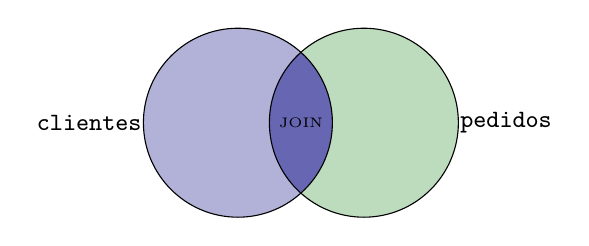
\begin{tikzpicture}
    \fill[NavyBlue!30] (0,0) circle (1.2);
    \fill[ForestGreen!30] (1.6,0) circle (1.2);
    \begin{scope}
      \clip (0,0) circle (1.2);
      \fill[NavyBlue!60] (1.6,0) circle (1.2);
    \end{scope}
    \draw (0,0) circle (1.2) node[left=1.1cm] {\small\texttt{clientes}};
    \draw (1.6,0) circle (1.2) node[right=1.1cm] {\small\texttt{pedidos}};
    \node at (0.8,0) {\tiny JOIN};
  \end{tikzpicture}
\end{center}

\textbf{Sintaxis general:}

\begin{lstlisting}[style=sql, caption={Sintaxis de INNER JOIN}]
SELECT columnas
FROM tabla_izquierda
INNER JOIN tabla_derecha
    ON tabla_izquierda.clave = tabla_derecha.clave;
\end{lstlisting}

\begin{ejemplo}
  Obtener los pedidos junto con el nombre del cliente que los realizó:

  \begin{lstlisting}[style=sql, caption={INNER JOIN entre clientes y pedidos}]
SELECT c.nombre,
       p.pedido_id,
       p.monto
FROM clientes AS c
INNER JOIN pedidos AS p
    ON c.cliente_id = p.cliente_id;
  \end{lstlisting}

  \textbf{Resultado:}

  \begin{center}
    \begin{tabular}{>{\ttfamily}l >{\ttfamily}c >{\ttfamily}r}
      \toprule
      \textbf{nombre}  & \textbf{pedido\_id} & \textbf{monto} \\
      \midrule
      Ana García  & 101 & 350.00 \\
      Luis Pérez  & 102 & 120.50 \\
      Luis Pérez  & 103 &  89.00 \\
      \bottomrule
    \end{tabular}
  \end{center}

  Los clientes \texttt{María López} y \texttt{Carlos Ruiz} no aparecen porque no tienen
  pedidos. El pedido \texttt{104} tampoco aparece porque su \texttt{cliente\_id = 5}
  no existe en \texttt{clientes}.
\end{ejemplo}

\begin{nota}
  La palabra clave \texttt{INNER} es opcional; \texttt{JOIN} a secas equivale a
  \texttt{INNER JOIN} en todos los motores SQL principales.
\end{nota}

% ─────────────────────────────────────────────────────────
\subsection{\texttt{LEFT JOIN}}

\begin{definicion}{LEFT JOIN}
  Devuelve \textbf{todas las filas de la tabla izquierda} más las coincidencias de la tabla
  derecha. Cuando no existe par, las columnas de la tabla derecha se rellenan con
  \texttt{NULL}.
\end{definicion}

\begin{center}
  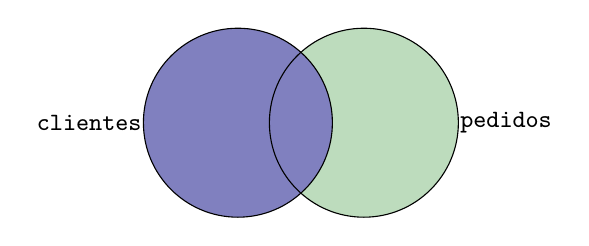
\begin{tikzpicture}
    \fill[NavyBlue!50] (0,0) circle (1.2);
    \fill[ForestGreen!30] (1.6,0) circle (1.2);
    \begin{scope}
      \clip (0,0) circle (1.2);
      \fill[NavyBlue!50] (1.6,0) circle (1.2);
    \end{scope}
    \draw (0,0) circle (1.2) node[left=1.1cm] {\small\texttt{clientes}};
    \draw (1.6,0) circle (1.2) node[right=1.1cm] {\small\texttt{pedidos}};
  \end{tikzpicture}
\end{center}

\textbf{Sintaxis general:}

\begin{lstlisting}[style=sql, caption={Sintaxis de LEFT JOIN}]
SELECT columnas
FROM tabla_izquierda
LEFT JOIN tabla_derecha
    ON tabla_izquierda.clave = tabla_derecha.clave;
\end{lstlisting}

\begin{ejemplo}
  Listar todos los clientes y, si tienen pedidos, mostrar su monto:

  \begin{lstlisting}[style=sql, caption={LEFT JOIN: todos los clientes con sus pedidos}]
SELECT c.nombre,
       p.pedido_id,
       p.monto
FROM clientes AS c
LEFT JOIN pedidos AS p
    ON c.cliente_id = p.cliente_id;
  \end{lstlisting}

  \textbf{Resultado:}

  \begin{center}
    \begin{tabular}{>{\ttfamily}l >{\ttfamily}c >{\ttfamily}r}
      \toprule
      \textbf{nombre}  & \textbf{pedido\_id} & \textbf{monto} \\
      \midrule
      Ana García   & 101  & 350.00 \\
      Luis Pérez   & 102  & 120.50 \\
      Luis Pérez   & 103  &  89.00 \\
      María López  & NULL &   NULL \\
      Carlos Ruiz  & NULL &   NULL \\
      \bottomrule
    \end{tabular}
  \end{center}

  Los clientes sin pedidos aparecen con \texttt{NULL} en las columnas de \texttt{pedidos}.
\end{ejemplo}

\textbf{Caso de uso habitual — detectar huérfanos:}

\begin{lstlisting}[style=sql, caption={Clientes que nunca han realizado un pedido}]
SELECT c.nombre
FROM clientes AS c
LEFT JOIN pedidos AS p
    ON c.cliente_id = p.cliente_id
WHERE p.pedido_id IS NULL;
\end{lstlisting}

% ─────────────────────────────────────────────────────────
\subsection{\texttt{RIGHT JOIN}}

\begin{definicion}{RIGHT JOIN}
  Devuelve \textbf{todas las filas de la tabla derecha} más las coincidencias de la tabla
  izquierda. Las columnas de la tabla izquierda se rellenan con \texttt{NULL} cuando no
  existe par. Es el simétrico de \texttt{LEFT JOIN}.
\end{definicion}

\begin{center}
  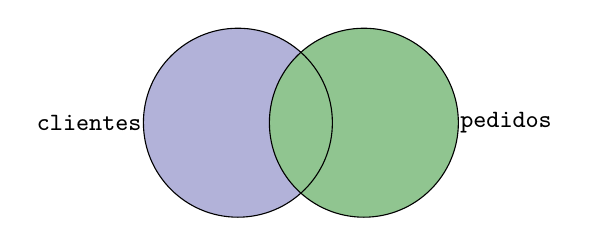
\begin{tikzpicture}
    \fill[NavyBlue!30] (0,0) circle (1.2);
    \fill[ForestGreen!50] (1.6,0) circle (1.2);
    \begin{scope}
      \clip (1.6,0) circle (1.2);
      \fill[ForestGreen!50] (0,0) circle (1.2);
    \end{scope}
    \draw (0,0) circle (1.2) node[left=1.1cm] {\small\texttt{clientes}};
    \draw (1.6,0) circle (1.2) node[right=1.1cm] {\small\texttt{pedidos}};
  \end{tikzpicture}
\end{center}

\textbf{Sintaxis general:}

\begin{lstlisting}[style=sql, caption={Sintaxis de RIGHT JOIN}]
SELECT columnas
FROM tabla_izquierda
RIGHT JOIN tabla_derecha
    ON tabla_izquierda.clave = tabla_derecha.clave;
\end{lstlisting}

\begin{ejemplo}
  Mostrar todos los pedidos e incluir el nombre del cliente si existe:

  \begin{lstlisting}[style=sql, caption={RIGHT JOIN: todos los pedidos con datos del cliente}]
SELECT c.nombre,
       p.pedido_id,
       p.monto
FROM clientes AS c
RIGHT JOIN pedidos AS p
    ON c.cliente_id = p.cliente_id;
  \end{lstlisting}

  \textbf{Resultado:}

  \begin{center}
    \begin{tabular}{>{\ttfamily}l >{\ttfamily}c >{\ttfamily}r}
      \toprule
      \textbf{nombre}  & \textbf{pedido\_id} & \textbf{monto} \\
      \midrule
      Ana García  & 101 & 350.00 \\
      Luis Pérez  & 102 & 120.50 \\
      Luis Pérez  & 103 &  89.00 \\
      NULL        & 104 & 200.00 \\
      \bottomrule
    \end{tabular}
  \end{center}

  El pedido \texttt{104} aparece con \texttt{NULL} en \texttt{nombre} porque su
  \texttt{cliente\_id = 5} no existe en la tabla \texttt{clientes}.
\end{ejemplo}

\begin{nota}
  En la práctica, \texttt{RIGHT JOIN} se usa con menos frecuencia que \texttt{LEFT JOIN}.
  Cualquier consulta con \texttt{RIGHT JOIN} puede reescribirse como un \texttt{LEFT JOIN}
  intercambiando el orden de las tablas:
  \begin{center}
    \texttt{A RIGHT JOIN B} $\equiv$ \texttt{B LEFT JOIN A}
  \end{center}
\end{nota}

% ─────────────────────────────────────────────────────────
\subsection{\texttt{UNION}}

\begin{definicion}{UNION}
  Combina verticalmente los resultados de dos o más sentencias \texttt{SELECT}.
  \texttt{UNION} elimina filas duplicadas; \texttt{UNION ALL} las conserva.
  Ambas consultas deben tener el \textbf{mismo número de columnas} y tipos de datos
  compatibles.
\end{definicion}

\textbf{Sintaxis general:}

\begin{lstlisting}[style=sql, caption={Sintaxis de UNION / UNION ALL}]
SELECT columna1, columna2, ...
FROM tabla_a
UNION [ALL]
SELECT columna1, columna2, ...
FROM tabla_b;
\end{lstlisting}

\begin{ejemplo}
  Obtener una lista unificada de correos de dos tablas distintas (\texttt{clientes} y
  \texttt{proveedores}), sin duplicados:

  \begin{lstlisting}[style=sql, caption={UNION de correos de clientes y proveedores}]
SELECT nombre, correo, 'cliente'   AS origen
FROM clientes
UNION
SELECT nombre, correo, 'proveedor' AS origen
FROM proveedores
ORDER BY nombre;
  \end{lstlisting}
\end{ejemplo}

\begin{ejemplo}
  Comparación entre \texttt{UNION} y \texttt{UNION ALL}:

  \begin{lstlisting}[style=sql, caption={Diferencia entre UNION y UNION ALL}]
-- Elimina duplicados (más lento: realiza ORDER + DISTINCT internamente)
SELECT ciudad FROM clientes
UNION
SELECT ciudad FROM proveedores;

-- Conserva duplicados (más rápido: no realiza deduplicación)
SELECT ciudad FROM clientes
UNION ALL
SELECT ciudad FROM proveedores;
  \end{lstlisting}
\end{ejemplo}

\begin{nota}
  Los nombres de las columnas del resultado se toman del \textbf{primer} \texttt{SELECT}.
  La cláusula \texttt{ORDER BY} solo puede aparecer \textbf{una vez}, al final de toda la
  sentencia, y afecta al conjunto combinado completo.
\end{nota}

% ── Tabla resumen ─────────────────────────────────────────
\subsection*{Resumen comparativo}

\begin{table}[H]
  \centering
  \caption{Comparación de operaciones de combinación en SQL}
  \renewcommand{\arraystretch}{1.3}
  \rowcolors{2}{gray!10}{white}
  \begin{tabularx}{\textwidth}{>{\ttfamily}l X X}
    \toprule
    \textbf{Operación}  & \textbf{Filas incluidas}                                   & \textbf{Uso típico}                         \\
    \midrule
    INNER JOIN  & Solo las que tienen coincidencia en ambas tablas             & Datos relacionados que siempre existen      \\
    LEFT JOIN   & Todas las de la tabla izquierda + coincidencias              & Encontrar registros sin par (huérfanos)     \\
    RIGHT JOIN  & Todas las de la tabla derecha + coincidencias                & Simétrico de LEFT JOIN                      \\
    UNION       & Filas de ambos SELECT, sin duplicados                        & Consolidar datos de tablas similares        \\
    UNION ALL   & Filas de ambos SELECT, con duplicados                        & Igual que UNION pero más eficiente          \\
    \bottomrule
  \end{tabularx}
\end{table}

